\documentclass[aspectratio=1610,12pt,xcolor=dvipsnames]{beamer}
\mode<presentation>

% Respect chosen fonts (serif) and metrics
\usefonttheme{professionalfonts}
\renewcommand{\familydefault}{\rmdefault}

% Figures
\usepackage{graphicx}
\usepackage{float}
\usepackage{tikz}
\usetikzlibrary{arrows.meta, positioning, fit}

%% table
\usepackage{xcolor}
\usepackage{fancyhdr}
\usepackage{booktabs}
\usepackage[table]{xcolor}

% subsection page template
\setbeamertemplate{subsection page}
{
  \begin{centering}
    \vfill
    {\usebeamerfont{section title}\usebeamercolor[fg]{section title}\Large\insertsubsectionhead\par}
    \vfill
  \end{centering}
}
% section page template
\setbeamertemplate{section page}
{
  \begin{centering}
    \vfill
    {\usebeamerfont{section title}\usebeamercolor[fg]{section title}\Large\insertsectionhead\par}
    \vfill
  \end{centering}
}

%% footnote
\setbeamertemplate{footnote}{%
  \parindent 0em\noindent%
  \raggedright\insertfootnotemark\insertfootnotetext\par%
}

%% theme
\usetheme{default}
\useoutertheme{miniframes}
\definecolor{nagivation}{rgb}{0,0,0.35} % (typo kept if intentional)
\definecolor{main}{rgb}{0,0,0.5}
\setbeamercolor{structure}{bg=white,fg=nagivation}
\setbeamercolor{frametitle}{fg=nagivation}
\setbeamercolor{section in head/foot}{fg=white,bg=nagivation}
\setbeamertemplate{footline}[page number]
\setbeamertemplate{items}[circle]
\setbeamerfont{footnote}{size=\footnotesize}
\setbeamerfont{caption}{size=\footnotesize}
\setbeamertemplate{subsection in head/foot}{}%
\setbeamertemplate{subsection in head/foot shaded}{}%

%% font
\usepackage{dsfont}
\usepackage{newpxtext}
\usepackage{newpxmath}
\usepackage{amsmath}

% Math & bib
\usepackage{amsmath,amsfonts,amssymb,bm}
\DeclareMathOperator*{\argmin}{arg\,min}
\newcommand{\indep}{\perp\!\!\!\, \perp}
\usepackage{natbib}
\bibliographystyle{asr}
\setcitestyle{aysep={}}
\usepackage[english]{babel}

\makeatletter
\DeclareRobustCommand\citep
{\begingroup\scriptsize\color{gray}\NAT@swatrue\let\NAT@ctype\z@\NAT@partrue
    \@ifstar{\NAT@fulltrue\NAT@citetp}{\NAT@fullfalse\NAT@citetp}}
\makeatother

% Roman numerals macro
\newcommand{\rom}[1]{\uppercase\expandafter{\romannumeral #1\relax}}

%% Title
\title[CML]{SOC 690S: Machine Learning in Causal Inference\\[1.5pt]}
\subtitle{\large Week 5: Causal Inference from Directed Acyclic Graphs \\[-10pt]}

%% author
\author[Jiang] 
{\large Wenhao Jiang\vspace{-2em}}

%% affiliation
\institute[Duke]{}
\titlegraphic{
\includegraphics[height=1.4cm]{Misc/duke_logo.png}}

\date[Duke]
{\large Department of Sociology, Fall 2025}

\begin{document}

%%%%%%%%%%%%%%%%%%%%%%%%%%%%%%%%%%%%
%%%%%%%%Begin Main Content%%%%%%%%%%
%%%%%%%%%%%%%%%%%%%%%%%%%%%%%%%%%%%%

%% Title page %%
\begin{frame}
    \titlepage 
\end{frame}

\begin{frame}{}
\vspace{-1.4em}
\setlength{\tabcolsep}{1pt}
{\footnotesize\begin{table}[h!]
\centering
\begin{tabular}{@{}llp{9.8cm}cc@{}}
\hline \hline\\[-10pt]
\textbf{\textcolor{black}{Week}} & \textbf{\textcolor{black}{Date}} & \textbf{\textcolor{black}{Topic}} & \multicolumn{2}{c@{}}{\textbf{\textcolor{black}{Problem sets}}} \\
 & & & Assign & Due \\
\hline \\[-10pt]
1  & Aug 26  & Introduction: Motivation and Linear Regression &  &  \\
2  & Sep 2  & Foundation: Machine Learning Basics &  &  \\
3  & Sep 9  & Foundation: Machine Learning Advanced & 1 &  \\
4  & Sep 16  &  Foundation: Causal Inference Basics &  &  \\
5  & Sep 23  & Foundation: Causal Inference Advanced & 2 & 1 \\[4pt]
\arrayrulecolor{gray}
\hline \\[-9pt]
6  & Sep 30  & Core: PSM and Doubly Robust Estimation & & \\
8  & Oct 7    & Core: Instrumental Variable Estimation & 3 & 2  \\
7  & Oct 14  & \textit{Fall break} &  &  \\
9  & Oct 21  & \textbf{In-class midterm} &  & \\
10  & Oct 28  &  Core: Regression Discontinuity Design &  4 & 3 \\
11  & Nov 4  & Core: Panel Data and Difference-in-Difference & & \\[4pt]
\arrayrulecolor{gray}
\hline \\[-9pt]
12  & Nov 11    & Advanced: Heterogeneous Treatment Effect & 5 & 4 \\
13 & Nov 18    & Advanced: Unstructured Data Feature Engineering & & \\
14 & Nov 25   & Advanced: Causal Reasoning in Machine Learning &  & 5 \\
 & Dec 13   & \textbf{Take-home final} & & \\
\arrayrulecolor{black}
\hline \hline
\end{tabular}
\end{table}}
\end{frame}

\section{Causal Inference via Linear Structural Equations}

\begin{frame}
  \sectionpage
\end{frame}

\begin{frame}{Structural Equation Model for Causal Inference}

\begin{itemize}
    \item Early conceptions of causality, most notably by Sewall Wright (a geneticist), used a \textit{structural} approach to link variables
    \begin{figure}
        \centering
        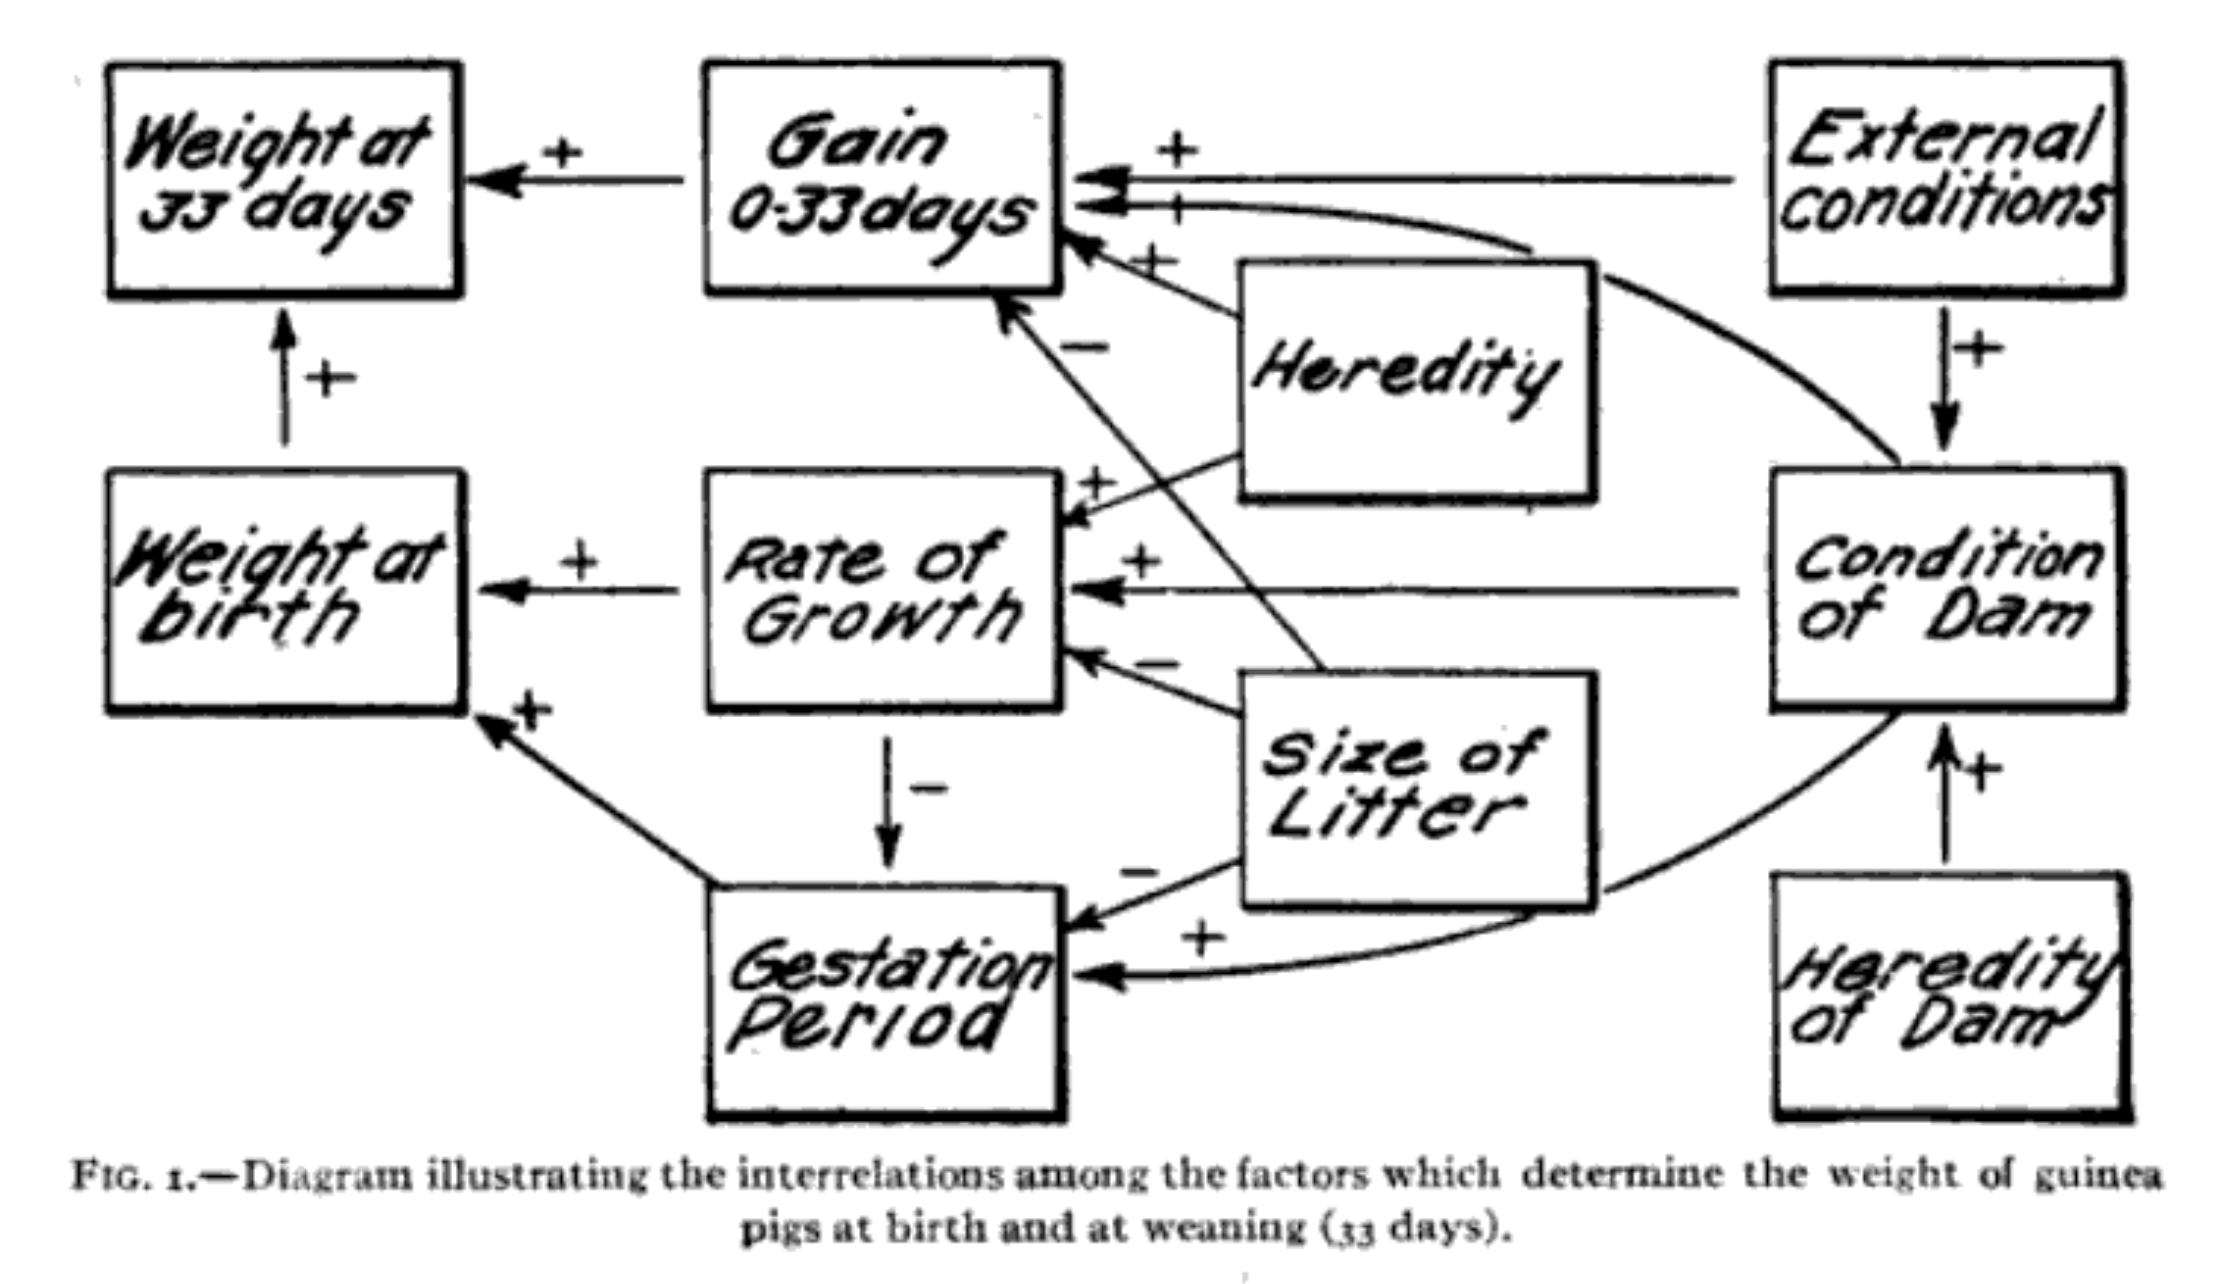
\includegraphics[width=0.83\linewidth]{Causal Inference DAGs/Figures/S.Wright.png}
    \end{figure}
\end{itemize}
\end{frame}

\begin{frame}{Structural Equation Model for Causal Inference}

\begin{itemize}
    \item This \textit{structural} approach became known as \textit{path analysis}, though most researchers did not interpret it under the framework of potential outcome
    \item Sociologists such as Peter M. Blau and Otis Dudley Duncan carried forward \textit{path analysis} in the mid- and late-20th century
    \begin{figure}
        \centering
        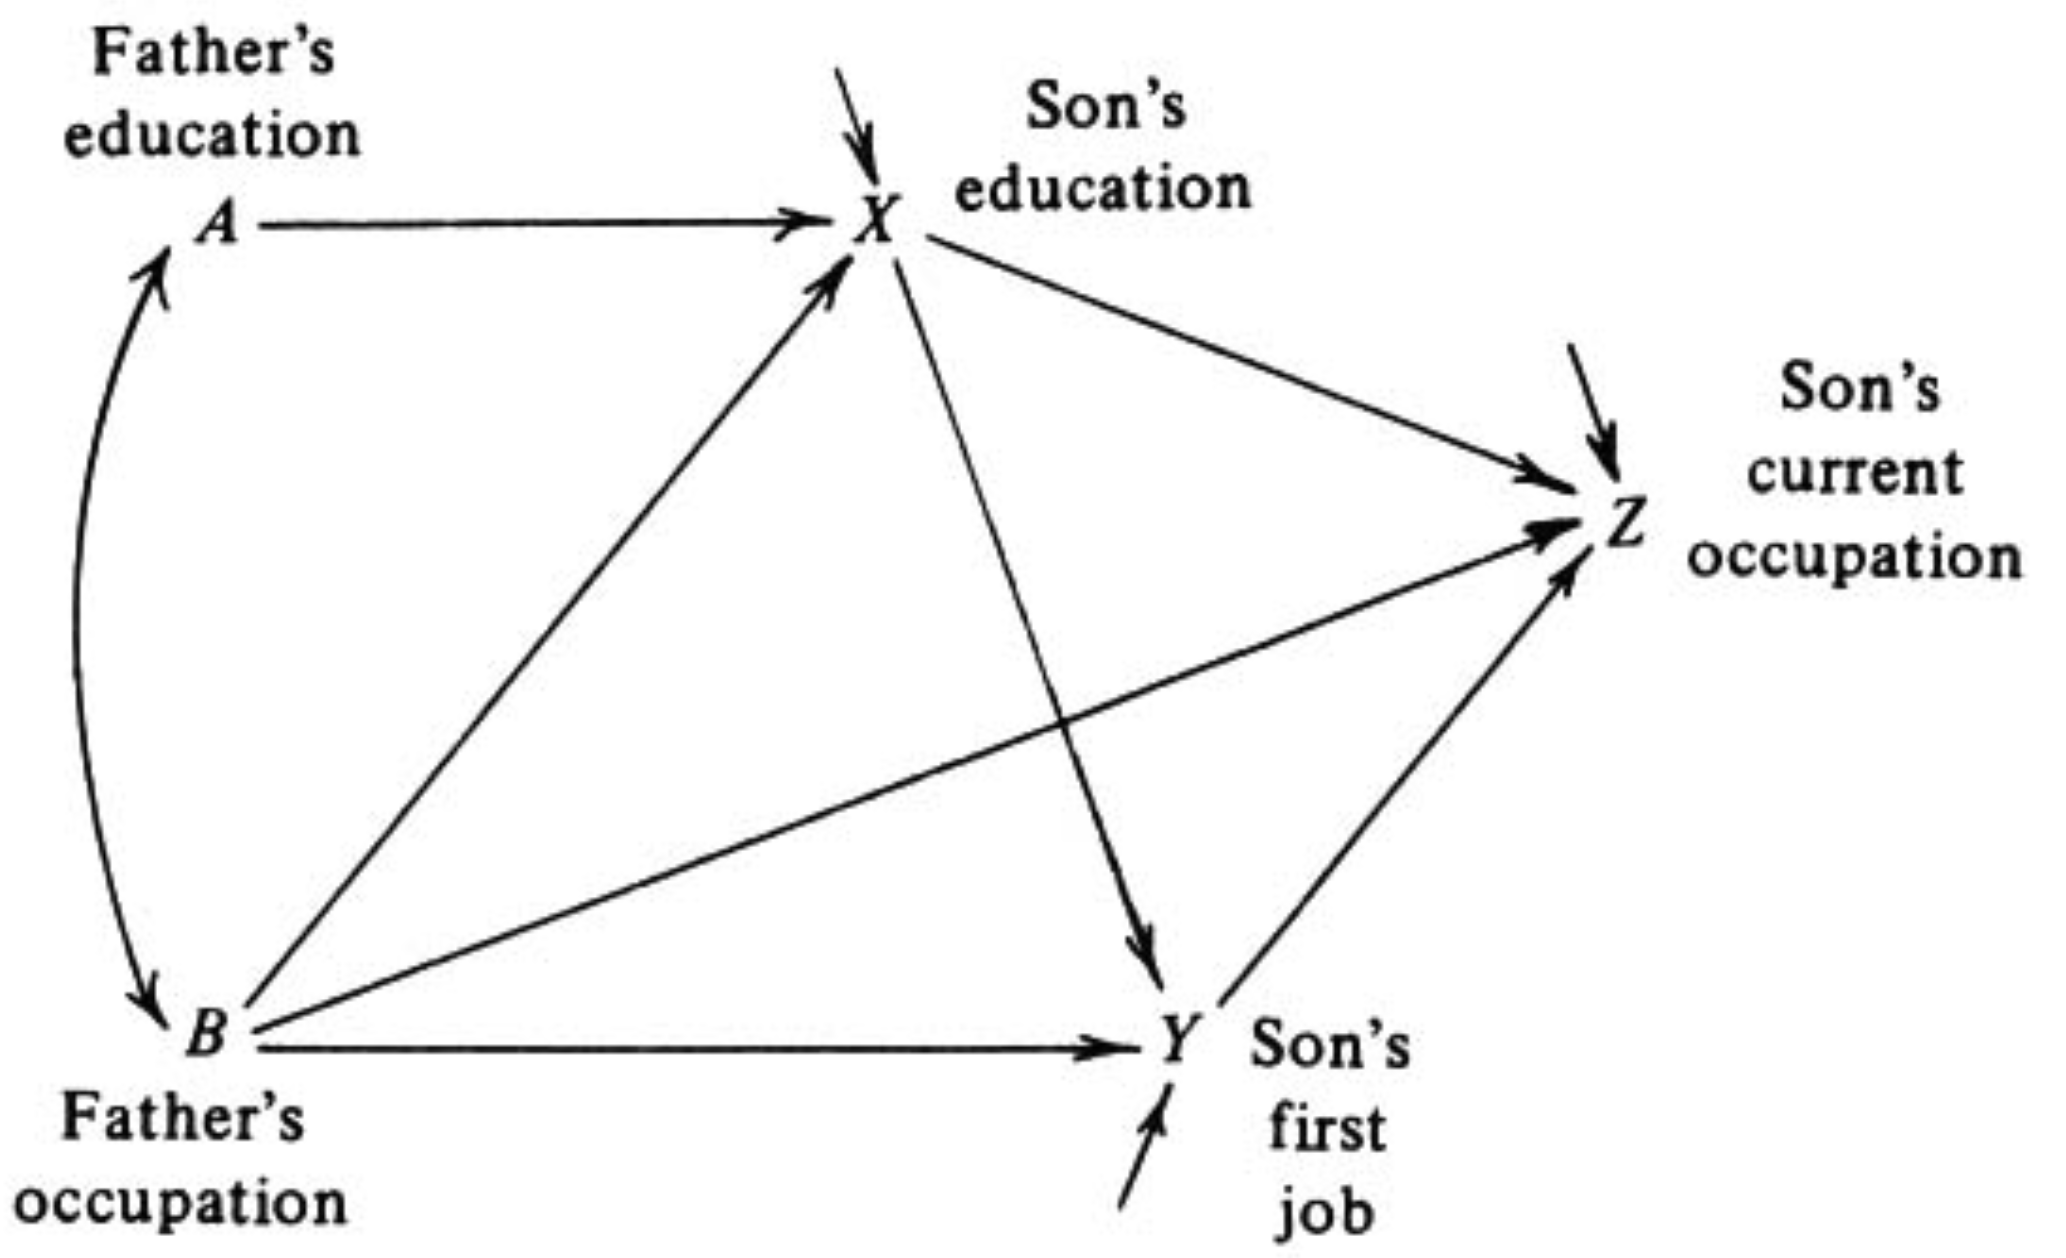
\includegraphics[width=0.62\linewidth]{Causal Inference DAGs/Figures/BlauDuncan.png}
    \end{figure}
\end{itemize}
\end{frame}

\begin{frame}{Structural Equation Model for Causal Inference}

\begin{itemize}
    \item Most applied researchers who used \textit{path analysis} did not interpret it under the potential outcome framework for causal identification
    \item Judea Pearl introduced a formal graphical language (\textit{directed acyclic graphs}, or DAG) in the 90s that linked \textit{structural equation models} to precise rules for causal identification
    \item Pearl’s framework provided clear conditions (\textit{e.g.}, backdoor and frontdoor criteria) that determine when causal effects are identifiable from observational data
    \item We will start from a simple \textit{structural equation model} to motivate the use of DAG
\end{itemize}
\end{frame}

\begin{frame}{A Simple Triangular Structural Equation Model}

\begin{itemize}
    \item We start with a simple model of a household's demand for gasoline
    \item We model log-demand $y$ given the log-price $p$
    \[y(p) := \delta p\]
    \item where $\delta$ is the elasticity of demand. Demand is random across households, and we may model this randomness as $U$—a stochastic shock that describes variation of demand across households
    \[Y(p) = \delta p + U, \quad E[U] = 0\]
    \item $Y(p)$ plays the \textit{same} role as Rubin's potential outcome, \textit{i.e.},
    \[E[Y(p_1) - Y(p_0)] = \delta(p_1 - p_0)\]
\end{itemize}
    
\end{frame}

\begin{frame}{A Simple Triangular Structural Equation Model}

\begin{itemize}
    \item We may want to introduce covariates to capture other observable factors that may be associated with demand
    \item We may think there are observable parts of the stochastic shock ($U$), characterized by $X$, which help predict household demand; $X$ may include family size, income, number of cars, or geographic location
    \[U = X'\beta + \epsilon_Y\]
    \item where $\epsilon_Y$ is independent of $X$ and has mean zero
    \[Y(p) := \delta p + X'\beta + \epsilon_Y , \quad \epsilon_Y \indep X \]
    \item This is a structural model of potential economic outcome; if log-price is set to $p$, then a household with $X$ can be predicted to purchase 
    $\delta p + X' \beta$ log-units of gasoline
\end{itemize}
\end{frame}

\begin{frame}{A Simple Triangular Structural Equation Model}

\begin{itemize}
    \item In reality, the observed log-price $P$ may depend on household characteristics $X$
    \[P(X) := X'v + \epsilon_p, \quad \epsilon_p \indep X \]
    \item where $\epsilon_p$ is independent of $X$ and has mean zero
    \item For example, households located in different regions would experience different gas prices
    \item $\epsilon_p \indep X$ assumes that household characteristics are determined well before gasoline prices faced by individual households are set
\end{itemize}
\end{frame}

\begin{frame}{A Simple Triangular Structural Equation Model}
    \begin{itemize}
        \item We also assume that households are otherwise \textit{price-takers}, meaning the observed $P$ is determined \textit{outside} of the model conditioning on $X$
        \item For example, log-price $P$ is independent of the stochastic shock of demand not captured by $X$
        \[P \indep \epsilon_Y \mid X \]
        \item This is the assumption of \textit{conditional exogeneity}—the econometric analog of \textit{conditional ignorability}
    \end{itemize}
\end{frame}

\begin{frame}{A Simple Triangular Structural Equation Model}
    \begin{itemize}
        \item Under these assumptions and equations, we have a triangular structural equation model (TSEM)
        \begin{align*}
            Y &:= \delta P + X'\beta + \epsilon_Y \\
            P &:= X' v + \epsilon_P \\
            X
        \end{align*}
        \item $\epsilon_Y$, $\epsilon_P$, and $X$ are mutually independent and determined \textit{outside of the model}
        \item In SEM, they are called \textit{exogeneous} variables
        \item $Y$ and $P$ are determined \textit{within} the model and are called the \textit{endogeneous} variables
    \end{itemize}
\end{frame}

\begin{frame}{A Simple Triangular Structural Equation Model}
    \begin{itemize}
        \item What do we mean by the model being \textit{structural}
        \item Each of the equation is assumed to model counterfactual scenarios
        \begin{align*}
            Y(p,x) &:= \delta p + x'\beta + \epsilon_Y \\
            P(x) &:= x' v + \epsilon_P
        \end{align*}
        \item The conceptual operation of ``setting'' the variables to their potential or counterfactual values is assumed to leave the structure intact
        \begin{itemize}
            \item The structural parameters are supposed to be invariant to changes in the distribution of exogeneous variables—$X$, $\epsilon_Y$, $\epsilon_P$—that have been generated outside of the model
        \end{itemize}
        \item We can therefore use these structural parameters to generate \textit{counterfactual} predictions
        \item The structural parameters $\delta$ and $v$ can be identified by linear regression
    \end{itemize}
\end{frame}

\subsection{From SEM to DAG}

\begin{frame}
  \subsectionpage
\end{frame}

\begin{frame}{From SEM to DAG}
    \begin{align*}
            Y &:= \delta P + X'\beta + \epsilon_Y \\
            P &:= X' v + \epsilon_P 
    \end{align*}
    
    \begin{itemize}
    \item This simple TSEM can be graphically depicted as a causal diagram
    \item Observed variables are shown as nodes, and causal paths are represented by directed arrows
    \end{itemize}
    \centering
    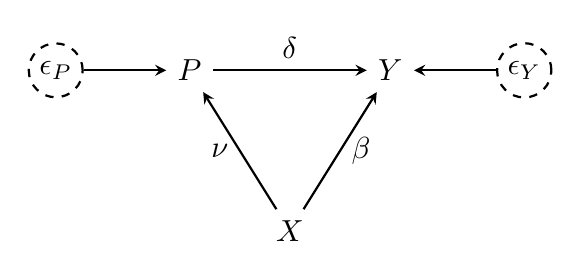
\begin{tikzpicture}[
    >=stealth,
    scale=0.85,
    thick,
    every node/.style={scale=1.1},
]
% Nodes
\node[circle,draw,dashed,inner sep=2pt] (eP) at (-2,0) {$\epsilon_P$};
\node (P) at (0,0) {$P$};
\node (X) at (1.5,-2.4) {$X$};
\node (Y) at (3,0) {$Y$};
\node[circle,draw,dashed,inner sep=2pt] (eY) at (5,0) {$\epsilon_Y$};
% Arrows
\draw[->] (eP) -- (P);
\draw[->] (P) -- node[above] {\fontsize{10}{12}\selectfont $\delta$} (Y);
\draw[->] (X) -- node[left] {\fontsize{10}{12}\selectfont $\nu$} (P);
\draw[->] (X) -- node[right] {\fontsize{10}{12}\selectfont $\beta$} (Y);
\draw[->] (eY) -- (Y);
    \end{tikzpicture}
\end{frame}

\begin{frame}{From SEM to DAG}

\begin{itemize}
    \item The graph initiates with the \textit{root nodes} $X$, $\epsilon_P$, $\epsilon_Y$
    \item The absence of links between the root nodes indicates orthogonality
    \item Understanding the orthogonality structure between nodes is an important input into identification of structural parameters through (linear) projection
    \item The nodes $X$ and $\epsilon_P$ are \textit{parents} of $P$; the nodes $P$, $X$, and $\epsilon_Y$ are \textit{parents} of $Y$
    \item The node $Y$ is a \textit{collider}, as two or more other variables (two causal arrows in the graph) ``collide'' at that variable
\end{itemize}
\end{frame}

\begin{frame}{From SEM to DAG}

\begin{itemize}
    \item The main effect of interest, $\delta$, or the structural causal effect of $P$ on $Y$, is identified after adjusting for $X$
    \[Y(p) := \delta p + X'\beta + \epsilon_Y , \quad \epsilon_Y \indep X, p \]
    \item In the language of the DAG, there are two paths connecting $P$ and $Y$
    \[P \rightarrow X \text{ and } P \leftarrow X \rightarrow Y \]
    \item The second path is called a \textit{backdoor path}—there is a common cause for $P$ and $Y$
    \item Figuratively speaking, controlling for $X$ is said to be ``closing the backdoor path'' (or satisfying the \textit{backdoor criterion}), shutting down the non-causal sources of statistical dependence between $P$ and $Y$
\end{itemize}
\end{frame}

\begin{frame}{From SEM to DAG}

\begin{itemize}
    \item Going back to the structural model; how do household characteristics impact gasoline demand
    \item The direct effect $\beta$ via $X \rightarrow Y$
    \item The indirect effect $v\delta$ via $X \rightarrow P \rightarrow Y$
    \item The total effect of $X$ on $Y$ is $v \delta + \beta$, which can be identified by projection of $Y$ on $X$
    \item There are no backdoor paths from $X$ to $Y$; no adjustments are needed to identify the total effect of $X$ on $Y$
\end{itemize}

\centering
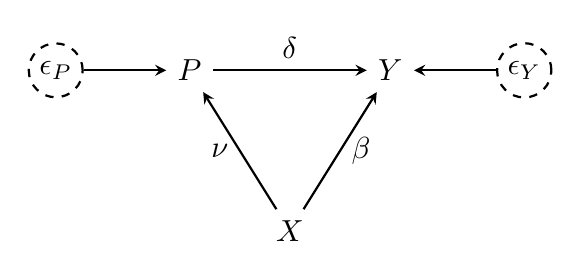
\begin{tikzpicture}[
    >=stealth,
    scale=0.85,
    thick,
    every node/.style={scale=1.1},
]
% Nodes
\node[circle,draw,dashed,inner sep=2pt] (eP) at (-2,0) {$\epsilon_P$};
\node (P) at (0,0) {$P$};
\node (X) at (1.5,-2.4) {$X$};
\node (Y) at (3,0) {$Y$};
\node[circle,draw,dashed,inner sep=2pt] (eY) at (5,0) {$\epsilon_Y$};
% Arrows
\draw[->] (eP) -- (P);
\draw[->] (P) -- node[above] {\fontsize{10}{12}\selectfont $\delta$} (Y);
\draw[->] (X) -- node[left] {\fontsize{10}{12}\selectfont $\nu$} (P);
\draw[->] (X) -- node[right] {\fontsize{10}{12}\selectfont $\beta$} (Y);
\draw[->] (eY) -- (Y);
\end{tikzpicture}
\end{frame}

\begin{frame}{From SEM to DAG}

\begin{itemize}
    \item We can also verify it by plugging in $P$
    \begin{align*}
        Y &= \delta (X'v + \epsilon_P) + X'\beta + \epsilon_Y \\
        &= (v\delta + \beta)'X + (\epsilon_Y + \delta \epsilon_P) \\
        \epsilon_Y + \delta \epsilon_P &\perp X
    \end{align*}
    \item Therefore, $v\delta + \beta$ coincides with the projection coefficient in the projection of $Y$ on $X$ \pause
    \item Conditioning on $P$ would allow us to identify the direct of $X$, \textit{i.e.}, $\beta$, but would prevent us from identifying the total effect $v\delta + \beta$
\end{itemize}

\end{frame}

\begin{frame}{The Backdoor Criterion}

\begin{itemize}
    \item A set of variables $Z$ satisfies the \textit{backdoor criterion} relative to an ordered pair of variables $(D,Y)$ in a DAG if
    \begin{itemize}
        \item No node in $Z$ is a descendant of $D$; and
        \item $Z$ blocks every path between $D$ and $Y$ that contains an arrow into $D$ (\textit{i.e.}, every ``backdoor path'' from $D$ to $Y$) \pause
    \end{itemize}
    \item If $Z$ satisfies the backdoor criterion, then the causal effect of $D$ on $Y$ is identifiable by conditioning on $Z$:
    \[
    P(Y(d)) = P(Y \mid do(D=d)) = \int P(Y \mid D=d, Z=z) f(z) dz
    \]
    \item $do(D=d)$ means that we intervene in the system and set $D=d$ as a potential treatment
    \item The distribution of the potential outcome $Y(d)$ is obtained by averaging the observed distribution of $Y$ among units with $D=d$ across strata of $Z$, weighted by the prevalence of each stratum
\end{itemize}
\end{frame}

\begin{frame}{From Backdoor Criterion to Conditional Ignorability}

\begin{itemize}
    \item The \textit{backdoor criterion} is closely linked with the potential outcome framework and the \textit{conditional ignorability} assumption
    \item Under \textit{conditional ignorability}, conditioning on covariates $X$ (\textit{i.e.}, within the same value or strata of $X$), treatments are as if randomly assigned
    \[D \indep Y(d) \mid X \]
    \item In reality, there could be a large array of covariates, and ``\textit{if `good' is taken to mean `best' fit, it is tempting to include anything in $X_i$ that helps predict treatment.}'' (\textcolor{nagivation}{Wooldridge, 2005})
    \item The \textit{backdoor criterion} provides the set of covariates to control for causal identification; its satisfaction is equivalent to fulfilling the \textit{conditional ignorability} assumption
\end{itemize}
\end{frame}

\begin{frame}{From Backdoor Criterion to Conditional Ignorability}
\begin{itemize}
    \item \textit{The First Law of Causal Inference}: DAGs (and corresponding SEM) is equivalent to the potential outcome framework
    \item In the above case (replacing $P$ by $D$ as a typical notation for treatment), conditioning on $X$ satisfies the \textit{backdoor criterion}
    \begin{align*}
        Y(d) &\indep D \mid X \\
        E[Y(d) \mid X] &= E[Y(d) \mid D=d,  X]
    \end{align*}
    \item This is also known as \textit{d-sepration}; conditioning on $X$ \textit{d-separates} the actual treatment $D$ and potential or counterfactual outcome $Y(d)$
\end{itemize}
\end{frame}

\begin{frame}{The Backdoor Criterion}

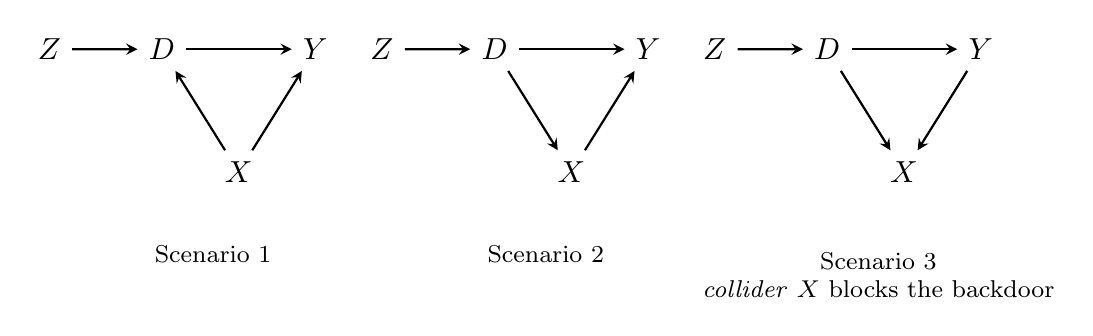
\begin{tikzpicture}[
>=stealth,
scale=0.65,
thick,
every node/.style={scale=1.1},
]
%% scenario 1
% nodes
\node (D) at (0,0) {$D$};
\node (X) at (1.5,-2.4) {$X$};
\node (Y) at (3,0) {$Y$};
\node (Z) at (-2.2,0) {$Z$};
% arrows
\draw[->] (Z) -- (D);
\draw[->] (D) -- node[above] {} (Y);
\draw[->] (X) -- node[left] {} (D);
\draw[->] (X) -- node[right] {} (Y);
\node at (1, -4) {\footnotesize{Scenario 1}}; \pause

%% scenario 2
% nodes
\node (D) at (6.5,0) {$D$};
\node (X) at (8,-2.4) {$X$};
\node (Y) at (9.5,0) {$Y$};
\node (Z) at (4.3,0) {$Z$};
% arrows
\draw[->] (Z) -- (D);
\draw[->] (D) -- node[above] {} (Y);
\draw[->] (D) -- node[left] {} (X);
\draw[->] (X) -- node[right] {} (Y);
\node at (7.5, -4) {\footnotesize Scenario 2}; \pause

%% scenario 3
% nodes
\node (D) at (13,0) {$D$};
\node (X) at (14.5,-2.4) {$X$};
\node (Y) at (16,0) {$Y$};
\node (Z) at (10.8,0) {$Z$};
% arrows
\draw[->] (Z) -- (D);
\draw[->] (D) -- node[above] {} (Y);
\draw[->] (D) -- node[left] {} (X);
\draw[->] (Y) -- node[right] {} (X);
\node[align=center, anchor=center, font=\footnotesize, yshift=-7pt] at (14,-4)
    {Scenario 3 \\ \textit{collider} $X$ blocks the backdoor};
\end{tikzpicture}
\end{frame}

\begin{frame}{The Backdoor Criterion}

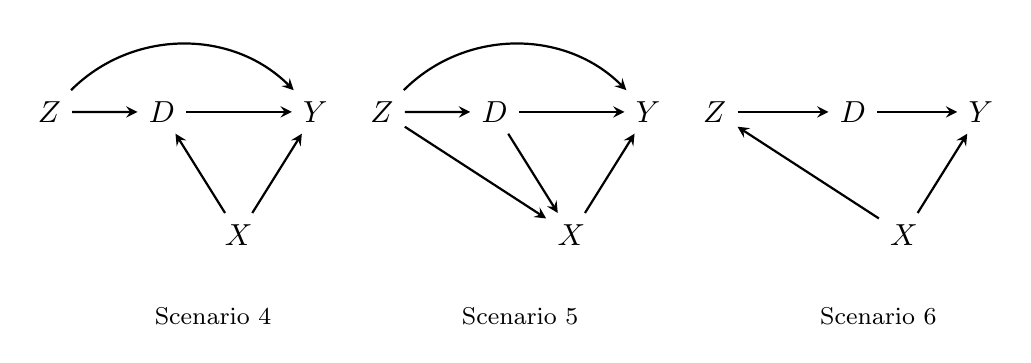
\begin{tikzpicture}[
>=stealth,
scale=0.65,
thick,
every node/.style={scale=1.1},
]
%% scenario 1
% nodes
\node (D) at (0,0) {$D$};
\node (X) at (1.5,-2.4) {$X$};
\node (Y) at (3,0) {$Y$};
\node (Z) at (-2.2,0) {$Z$};
% arrows
\draw[->] (Z) -- (D);
\draw[->] (Z) to[out=45,in=135] (Y);
\draw[->] (D) -- node[above] {} (Y);
\draw[->] (X) -- node[left] {} (D);
\draw[->] (X) -- node[right] {} (Y);
\node at (1, -4) {\footnotesize{Scenario 4}}; \pause

%% scenario 2
% nodes
\node (D) at (6.5,0) {$D$};
\node (X) at (8,-2.4) {$X$};
\node (Y) at (9.5,0) {$Y$};
\node (Z) at (4.3,0) {$Z$};
% arrows
\draw[->] (Z) -- (D);
\draw[->] (Z) -- (X);
\draw[->] (Z) to[out=45,in=135] (Y);
\draw[->] (D) -- node[above] {} (Y);
\draw[->] (D) -- node[left] {} (X);
\draw[->] (X) -- node[right] {} (Y);
\node at (7, -4) {\footnotesize Scenario 5}; \pause

%% scenario 3
% nodes
\node (D) at (13.5,0) {$D$};
\node (X) at (14.5,-2.4) {$X$};
\node (Y) at (16,0) {$Y$};
\node (Z) at (10.8,0) {$Z$};
% arrows
\draw[->] (Z) -- (D);
\draw[->] (D) -- node[above] {} (Y);
\draw[->] (X) -- node[left] {} (Z);
\draw[->] (X) -- node[right] {} (Y);
\node at (14, -4) {\footnotesize Scenario 6};
\end{tikzpicture}
\end{frame}

\begin{frame}{The Impact of 401(k) Eligibility on Financial Outcome}
\begin{itemize}
    \item 401(k) eligbility ($D$) might affect an individual's net financial assets ($Y$) both directly and indirectly through the employer's matching contribution ($M$)
    \item Worker-level ($X$) and firm-level ($F$) characteristics and latent factors ($U$) may additionally structure the model 
\end{itemize}

\centering
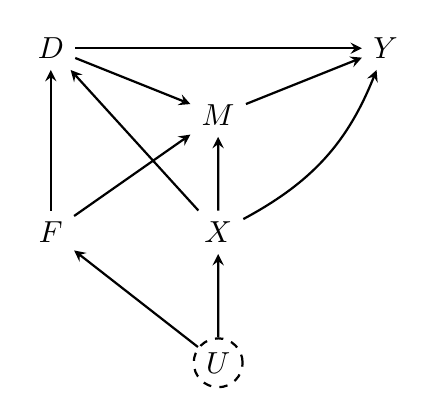
\begin{tikzpicture}[
    scale=0.85,
    thick,
    every node/.style={scale=1.1},
    node distance=4cm and 4cm,
    >=stealth
]

% Nodes placed manually in a grid
\node (D) at (0,4) {$D$};
\node (Y) at (5,4) {$Y$};
\node (F) at (0,1.25) {$F$};
\node (M) at (2.5,3) {$M$};
\node (X) at (2.5,1.25) {$X$};
\node[circle,draw,dashed,inner sep=2pt] (U) at (2.5,-0.7) {$U$};

% Arrows
\draw[->] (D) -- (Y);
\draw[->] (D) -- (M);
\draw[->] (X) -- (D);
\draw[->] (F) -- (D);
\draw[->] (F) -- (M);
\draw[->] (U) -- (F);
\draw[->] (U) -- (X);
\draw[->] (X) -- (M);
\draw[->, bend right=20] (X) to (Y);
\draw[->] (M) -- (Y);
\end{tikzpicture}
\end{frame}


\begin{frame}{Conditional Ignorability from DAG}

\begin{itemize}
    \item In the case of 401(k) eligibility on financial outcome, conditioning on $F$ and $X$ satisfies the \textit{backdoor criterion}
    \begin{align*}
        Y(d) &\indep D \mid F, X \\
        E[Y(d) \mid F, X] &= E[Y(d) \mid D=d, F, X]
    \end{align*}
    \item This is also known as \textit{d-sepration}; conditioning on $F$ and $X$ \textit{d-separates} the actual treatment $D$ and potential or counterfactual outcome $Y(d)$
\end{itemize}
\end{frame}

\begin{frame}{\textit{d-Separation} from DAG and Conditional Ignorability}

\begin{itemize}
    \item The \textit{actual} realization of treatment $D$ is still a function of $F$ and $X$
    \item $D$ is \textit{independent} of the potential outcome $Y(d)$ given $F$ and $X$
\end{itemize}

\centering
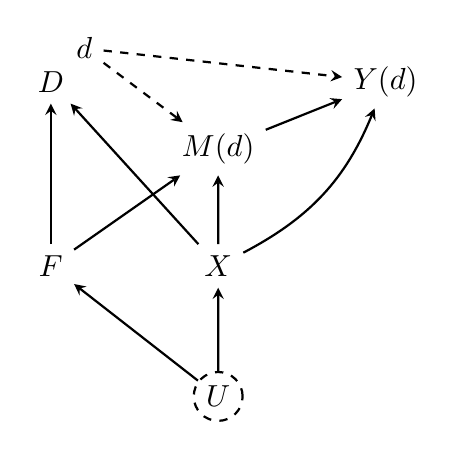
\begin{tikzpicture}[
    scale=0.85,
    thick,
    every node/.style={scale=1.1},
    node distance=4cm and 4cm,
    >=stealth
]

% Nodes placed manually in a grid
\node (D) at (0,4) {$D$};
\node (d) at (0.5,4.5) {$d$};
\node (Y) at (5,4) {$Y(d)$};
\node (F) at (0,1.25) {$F$};
\node (M) at (2.5,3) {$M(d)$};
\node (X) at (2.5,1.25) {$X$};
\node[circle,draw,dashed,inner sep=2pt] (U) at (2.5,-0.7) {$U$};

% Arrows
\draw[->,dashed] (d) -- (Y);
\draw[->,dashed] (d) -- (M);
\draw[->] (X) -- (D);
\draw[->] (F) -- (D);
\draw[->] (F) -- (M);
\draw[->] (U) -- (F);
\draw[->] (U) -- (X);
\draw[->] (X) -- (M);
\draw[->, bend right=20] (X) to (Y);
\draw[->] (M) -- (Y);
\end{tikzpicture}
\end{frame}

\subsection{When Conditioning Can Go Wrong: Collider Bias}

\begin{frame}
  \subsectionpage
\end{frame}

\begin{frame}{When Conditioning Can Go Wrong: Collider Bias}

\begin{itemize}
    \item Consider the following SEM
    \begin{align*}
        T &:= \epsilon_T \\
        B &:= \epsilon_B \\
        C &:= T + B + \epsilon_C
    \end{align*}
    \item where $\epsilon_T$, $\epsilon_B$, and $\epsilon_C$ are independent $\mathcal{N} (0,1)$ shocks; $E[T] = 0$, $E[T \mid B = b]= 0$
\end{itemize}

\centering
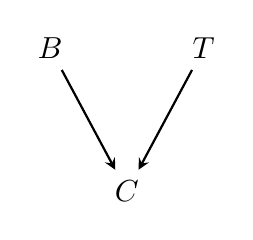
\begin{tikzpicture}[
>=stealth,
scale=0.65,
thick,
every node/.style={scale=1.1},
]
% nodes
\node (B) at (0,0) {$B$};
\node (C) at (1.5,-2.8) {$C$};
\node (T) at (3,0) {$T$};
% arrows
\draw[->] (B) -- node[left] {} (C);
\draw[->] (T) -- node[right] {} (C);
\end{tikzpicture}
\end{frame}

\begin{frame}{When Conditioning Can Go Wrong: Collider Bias}
\begin{itemize}
    \item Conditioning on \textit{collider} $C$ will create spurious dependence between $B$ and $T$;
    $E[T \mid B, C] \neq 0$
    \item Remember $T = C - B - \epsilon_C$, $E[T \mid B, C]$ is the predicted value of $T$ after linear projection of $T$ on $C-B$
    \begin{align*}
        E[T \mid B, C] &= \frac{Cov(T, (C-B))}{V(C-B)} (C-B) \\
        &= \frac{Cov(T,T+\epsilon_C)}{V(T+\epsilon_C)} (C-B) \\
        &= \frac{1}{2}(C-B)
    \end{align*}
\end{itemize}
\end{frame}

\begin{frame}{When Conditioning Can Go Wrong: Collider Bias}
    \begin{align*}
        E[T \mid B, C] &= E\left[E[T \mid B=b, C]\right] \\ 
        &= E\left[\frac{1}{2} (C-b) \right] \\
        &= -\frac{b}{2}
    \end{align*}

    \begin{itemize}
    \item Controlling for $C$, the predictive effect of $B$ on $T$ is $1/2$; this is \textit{not} a causal effect (spurious)
    \item This is the \textit{collider bias}, which is known as a form of sample selection bias (Heckman selection bias)
    \end{itemize}
\end{frame}

\begin{frame}{When Conditioning Can Go Wrong: Collider Bias}

\begin{itemize}
    \item Conditioning on a collider $C$ opens associations among its parents \textit{and all their ancestors}
\end{itemize}

\centering
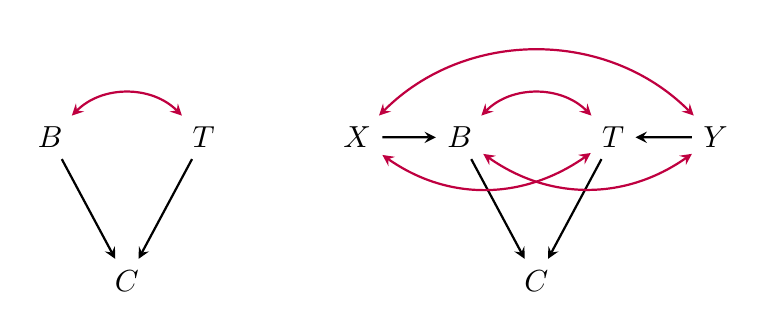
\begin{tikzpicture}[
>=stealth,
scale=0.65,
thick,
every node/.style={scale=1.1},
]
% nodes
\node (B) at (0,0) {$B$};
\node (C) at (1.5,-2.8) {$C$};
\node (T) at (3,0) {$T$};
% arrows
\draw[->] (B) -- node[left] {} (C);
\draw[->] (T) -- node[right] {} (C);
\draw[<->,color=purple] (B) to[out=45,in=135] (T);

% nodes
\node (B) at (8,0) {$B$};
\node (X) at (6,0) {$X$};
\node (C) at (9.5,-2.8) {$C$};
\node (T) at (11,0) {$T$};
\node (Y) at (13,0) {$Y$};
% arrows
\draw[->] (B) -- node[left] {} (C);
\draw[->] (X) -- (B);
\draw[->] (T) -- node[right] {} (C);
\draw[->] (Y) -- (T);
\draw[<->,color=purple] (B) to[out=45,in=135] (T);
\draw[<->,color=purple] (X) to[out=45,in=135] (Y);
\draw[<->,color=purple] (X) to[out=-35,in=-145] (T);
\draw[<->,color=purple] (B) to[out=-35,in=-145] (Y);
\end{tikzpicture}
\end{frame}

\begin{frame}{When Conditioning Can Go Wrong: Collider Bias}

\begin{itemize}
    \item In some cases, regression on a collider can be useful for \textit{predictive} tasks
    \item Suppose the preceding SEM provides a simplified version of actors and actresses in Hollywood
    \item $T$ denotes talent, $C$ celebrity (success or popularity), and $B$ bonhomie (approachability or friendliness
    \item Now if we condition on $C$ (say the person remains in Hollywood $C>0$), $B$ and $T$ will be \textit{negatively} correlated
    \item For those without bonhomie characters, they have to be very talented to remain in Hollywood; a prediction of talent is possible within Hollywood
\end{itemize}
\end{frame}

\begin{frame}{Collider Bias: Birth-Weight Paradox}

\begin{itemize}
    \item In a study conducted in 1991 in the US, it was found that infants born to smokers have:
    \begin{itemize}
        \item Higher risk of low birth-weight (LBW)
        \item Higher infant mortality
    \end{itemize}
    \item However, among infants with LBW, mortality is \textit{lower} for infants of smokers than for infants of non-smokers
    \item The naive interpretation is that smoking may be protective conditional on having LBW
    \item However, the more plausible explanation is LBW is a \textit{collider}
\end{itemize}
\end{frame}

\begin{frame}{Collider Bias: Birth-Weight Paradox}

\begin{itemize}
    \item $U$ could be unobserved competing risks that can cause LBW and higher mortality
\end{itemize}

\centering
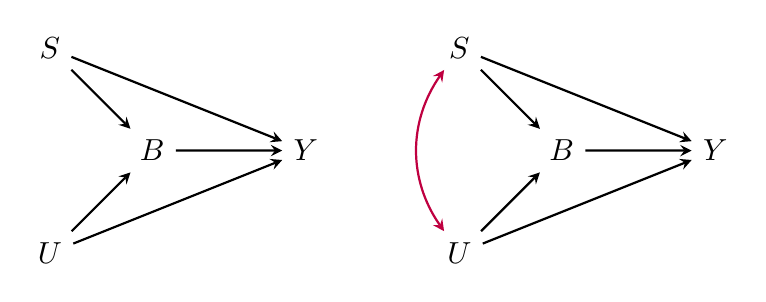
\begin{tikzpicture}[
>=stealth,
scale=0.65,
thick,
every node/.style={scale=1.1},
]
\node (S) at (0,0) {$S$};
\node (B) at (2,-2) {$B$};
\node (Y) at (5,-2) {$Y$};
\node (U) at (0,-4) {$U$};

% Arrows
\draw[->] (S) -- (B);
\draw[->] (S) -- (Y);
\draw[->] (U) -- (B);
\draw[->] (U) -- (Y);
\draw[->] (B) -- (Y);

\node (S) at (8,0) {$S$};
\node (B) at (10,-2) {$B$};
\node (Y) at (13,-2) {$Y$};
\node (U) at (8,-4) {$U$};

% Arrows
\draw[->] (S) -- (B);
\draw[->] (S) -- (Y);
\draw[->] (U) -- (B);
\draw[->] (U) -- (Y);
\draw[->] (B) -- (Y);
\draw[<->,color=purple] (S) to[out=-125,in=125] (U);

\end{tikzpicture}
\end{frame}

\begin{frame}{Collider Bias: Birth-Weight Paradox}
\vspace{-10pt}
\begin{align*}
    Y &:= S + B + \kappa U + \epsilon_Y \\
    B &:= S + U + \epsilon_B \\
    S &:= \epsilon_S \\
    U &:= \epsilon_U
\end{align*}
\begin{itemize}
    \item where $\epsilon_U$, $\epsilon_Y$, $\epsilon_S$, and $\epsilon_B$ are independent $\mathcal{N}(0,1)$ shocks
    \item If we project $Y$ on $S$, we recover the correct positive causal effect of 2
    \item However, when we project $Y$ on $S$ and $B$, we learn a CEF of the form
    \[E[Y \mid S, B] = S + B + (1-\kappa/2)S + (1+\kappa/2)B\]
    \item If the competing risks $U$ increase infant mortality a lot, \textit{i.e.}, $\kappa \gg 1$, the project recovers an erroneous large negative effect $1-\kappa/2$ of smoking on morality
\end{itemize}
\end{frame}

\begin{frame}{Collider Bias and Pearl's Classic Example}

\begin{itemize}
    \item We want to estimate the causal effect of $D$ on $Y$, \textit{i.e.}, the mapping $d \mapsto Y(d)$
\end{itemize}
\centering
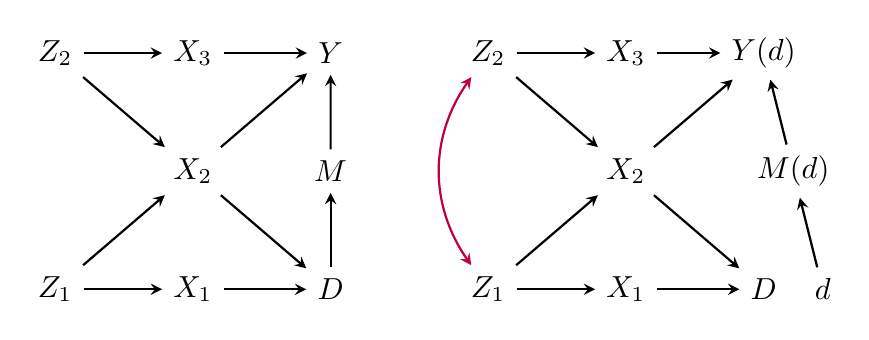
\begin{tikzpicture}[
    >=stealth,
    scale=0.5,
    thick,
    every node/.style={scale=1.1},
]

% Nodes
\node (Z2) at (0,6) {$Z_2$};
\node (Z1) at (0,0) {$Z_1$};
\node (X3) at (3.5,6) {$X_3$};
\node (X1) at (3.5,0) {$X_1$};
\node (X2) at (3.5,3) {$X_2$};
\node (D)  at (7,0) {$D$};
\node (M)  at (7,3) {$M$};
\node (Y)  at (7,6) {$Y$};

% Arrows
\draw[->] (Z2) -- (X3);
\draw[->] (Z2) -- (X2);
\draw[->] (Z1) -- (X1);
\draw[->] (Z1) -- (X2);
\draw[->] (X1) -- (D);
\draw[->] (X2) -- (D);
\draw[->] (X2) -- (Y);
\draw[->] (X3) -- (Y);
\draw[->] (D) -- (M);
\draw[->] (M) -- (Y); \pause

% Nodes
\node (Z2) at (11,6) {$Z_2$};
\node (Z1) at (11,0) {$Z_1$};
\node (X3) at (14.5,6) {$X_3$};
\node (X1) at (14.5,0) {$X_1$};
\node (X2) at (14.5,3) {$X_2$};
\node (D)  at (18,0) {$D$};
\node (Y)  at (18,6) {$Y(d)$};
\node (d) at (19.5,0) {$d$};
\node (Md) at (18.75,3) {$M(d)$};

% Arrows
\draw[->] (Z2) -- (X3);
\draw[->] (Z2) -- (X2);
\draw[->] (Z1) -- (X1);
\draw[->] (Z1) -- (X2);
\draw[->] (X1) -- (D);
\draw[->] (X2) -- (D);
\draw[->] (X2) -- (Y);
\draw[->] (X3) -- (Y);
\draw[->] (d) -- (Md);
\draw[->] (Md) -- (Y);
\draw[<->,color=purple] (Z2) to[out=-125,in=125] (Z1);
\end{tikzpicture}
\end{frame}

\section{Deeper Dive in DAG, Good and Bad Controls}
\begin{frame}
    \sectionpage
\end{frame}

\begin{frame}{Good and Bad Controls from DAG}

\begin{itemize}
    \item Sometimes we have causes of only treatment or only outcome
    \item In Scenario 1, including $Z$ can reduce estimation variance; in scenario 2, including $Z$ may increase estimation variance
\end{itemize}

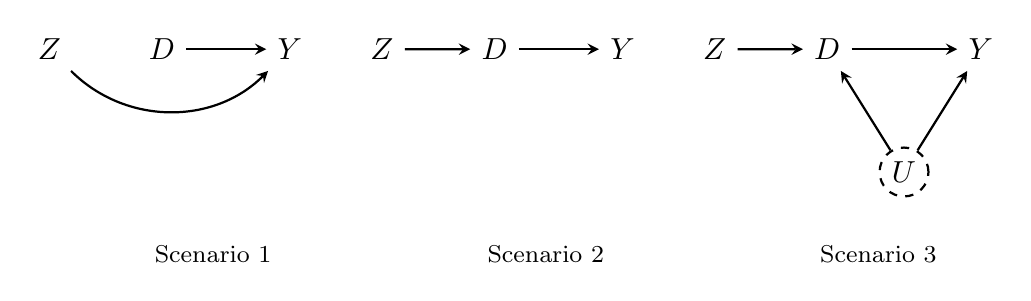
\begin{tikzpicture}[
>=stealth,
scale=0.65,
thick,
every node/.style={scale=1.1},
]
%% scenario 1
% nodes
\node (D) at (0,0) {$D$};
\node (Y) at (2.5,0) {$Y$};
\node (Z) at (-2.2,0) {$Z$};
% arrows
\draw[->] (D) -- node[above] {} (Y);
\draw[->] (Z) to[out=-45,in=-135] (Y);
\node at (1, -4) {\footnotesize{Scenario 1}};

%% scenario 2
% nodes
\node (D) at (6.5,0) {$D$};
\node (Y) at (9,0) {$Y$};
\node (Z) at (4.3,0) {$Z$};
% arrows
\draw[->] (Z) -- (D);
\draw[->] (D) -- node[above] {} (Y);
\node at (7.5, -4) {\footnotesize Scenario 2};

%% scenario 3
% nodes
\node (D) at (13,0) {$D$};
\node[circle,draw,dashed,inner sep=2pt] (U) at (14.5,-2.4) {$U$};
\node (Y) at (16,0) {$Y$};
\node (Z) at (10.8,0) {$Z$};
% arrows
\draw[->] (Z) -- (D);
\draw[->] (D) -- node[above] {} (Y);
\draw[->] (U) -- node[left] {} (D);
\draw[->] (U) -- node[right] {} (Y);
\node at (14,-4) {\footnotesize Scenario 3};
\end{tikzpicture}
\end{frame}

\begin{frame}{Good and Bad Controls: Single Cause}
    \begin{itemize}
    \item In scenario 3, adjusting for $Z$ can exacerbate the bias stemming from unobserved confounding
    \item Controlling for $Z$ removes exogeneous variation in the treatment $D$ that is useful for identifying the causal effect but leaves the confounded variation
    \item The resulting estimated effect may be essentially driven by the unobserved confounder and be heavily biased \pause
    \item Indeed, variables like $Z$ are known as \textit{instrumental} variables
    \item These variables can be thought as inducing natural experiments that can be leveraged for causal identification in the presence of unobserved confounding
    \item Importantly, instruments \textit{should not} be used in an identification by adjustment strategy
    \end{itemize}
\end{frame}

\begin{frame}{Good and Bad Controls: Post-Treatment Variables}

\begin{itemize}
    \item Explicitly adjusting for post-treatment variables is almost always a bad idea
    \item In many cases, post-treatment variables are included implicitly (and should be thought carefully) through \textit{e.g.}, data and sample collection and variable definition
    \item For example, when estimating the effect of education on wages using data on \textit{employed} individuals, we are implicitly conditioning on \textit{employment}, which is a post-treatment variable and can lead to selection bias
\end{itemize}
\end{frame}

\begin{frame}{Good and Bad Controls: Post-Treatment Variables}

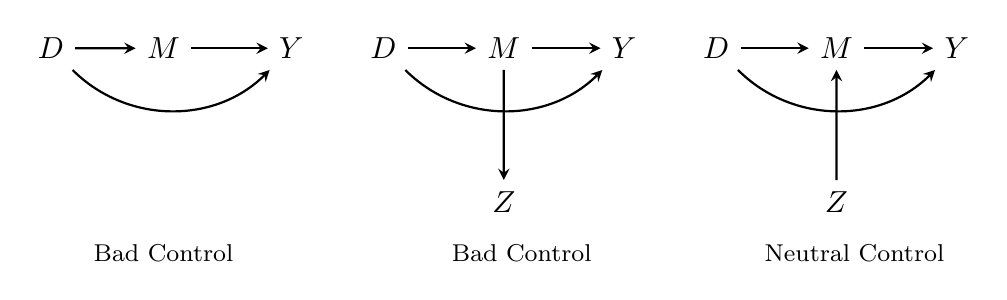
\begin{tikzpicture}[
>=stealth,
scale=0.65,
thick,
every node/.style={scale=1.1},
]
%% scenario 1
% nodes
\node (M) at (0,0) {$M$};
\node (Y) at (2.5,0) {$Y$};
\node (D) at (-2.2,0) {$D$};
% arrows
\draw[->] (D) -- (M);
\draw[->] (M) -- (Y);
\draw[->] (D) to[out=-45,in=-135] (Y);
\node at (0, -4) {\footnotesize{Bad Control}};

%% scenario 2
% nodes
\node (M) at (6.65,0) {$M$};
\node (Y) at (9,0) {$Y$};
\node (D) at (4.3,0) {$D$};
\node (Z) at (6.65,-3) {$Z$};
% arrows
\draw[->] (D) -- (M);
\draw[->] (M) -- (Y);
\draw[->] (M) -- (Z);
\draw[->] (D) to[out=-45,in=-135] (Y);
\node at (7, -4) {\footnotesize{Bad Control}};

%% scenario 3
% nodes
\node (M) at (13.15,0) {$M$};
\node (Y) at (15.5,0) {$Y$};
\node (D) at (10.8,0) {$D$};
\node (Z) at (13.15,-3) {$Z$};
% arrows
\draw[->] (D) -- (M);
\draw[->] (M) -- (Y);
\draw[->] (Z) -- (M);
\draw[->] (D) to[out=-45,in=-135] (Y);
\node at (13.5, -4) {\footnotesize{Neutral Control}};
\end{tikzpicture}
\end{frame}

\begin{frame}{Good and Bad Controls: Post-Treatment Variables}

\begin{itemize}
    \item $M$ is a bad control even for the \textit{controlled direct effect}
    \item Outcome of the outcome is also a bad control
\end{itemize}

\centering
\begin{tikzpicture}[
>=stealth,
scale=0.65,
thick,
every node/.style={scale=1.1},
]
% nodes
\node (M) at (0,0) {$M$};
\node[circle,draw,dashed,inner sep=2pt] (U) at (1.5,-2.4) {$U$};
\node (Y) at (3,0) {$Y$};
\node (D) at (-3,0) {$D$};
% arrows
\draw[->] (M) -- node[above] {} (Y);
\draw[->] (U) -- node[left] {} (M);
\draw[->] (D) -- node[left] {} (M);
\draw[->] (U) -- node[right] {} (Y);
\draw[->] (D) to[out=45,in=135] (Y);

% nodes
\node (Y) at (9,0) {$Y$};
\node (Z) at (11.5,0) {$Z$};
\node (D) at (6.5,0) {$D$};
% arrows
\draw[->] (Y) -- node[above] {} (Z);
\draw[->] (D) -- node[left] {} (Y);
\end{tikzpicture}
    
\end{frame}

\section{Front-Door Criterion}
\begin{frame}
    \sectionpage
\end{frame}

\begin{frame}{The Front-Door Criterion}

\centering
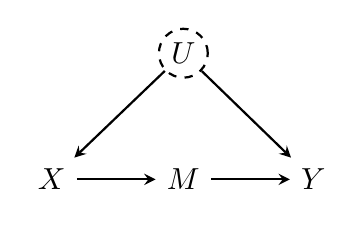
\begin{tikzpicture}[
>=stealth,
scale=0.65,
thick,
every node/.style={scale=1.1},
]
\node (X) {$X$};
\node[right=of X] (M) {$M$};
\node[right=of M] (Y) {$Y$};
\node[above=1cm of M,circle,draw,dashed,inner sep=2pt] (U) {$U$};

\draw[->] (X) -- (M);
\draw[->] (M) -- (Y);
\draw[->, bend left=25] (U) -- (X);
\draw[->, bend right=25] (U) -- (Y);
\end{tikzpicture}

\begin{itemize}
    \item The frontdoor criterion has the following setup 
    \begin{itemize}
        \item All directed paths from $X$ to $Y$ go through $M$
        \item There is \textit{no} unblocked backdoor paths from $X$ to $M$
        \item All backdoor paths from $M$ to $Y$ are blocked by $X$
    \end{itemize}
\end{itemize}
\end{frame}

\begin{frame}{The Front-Door Criterion}
    \begin{itemize}
    \item The causal effect of $X$ on $Y$ is then given by
    \begin{align*}
    P(Y(x)) 
    &= P(Y \mid do(X=x)) \\
    &= \sum_m P(Y \mid do(X=x), M=m)\, P(M=m \mid do(X=x)) \\
    &= \sum_m P(Y \mid do(M=m))\, P(M=m \mid X=x) \\
    &= \sum_m P(M=m \mid X=x)\,
       \left[ \sum_{x'} P(Y \mid M=m, X=x')\, P(X=x') \right]
    \end{align*}
    \end{itemize}
\end{frame}

\begin{frame}{The Front-Door Criterion: The APC Problem}

\begin{itemize}
    \item Standard APC regression:
\[
Y_{it} = \alpha + \beta_A \, A_i + \beta_P \, P_t + \beta_C \, C_i + \epsilon_{it}
\]

\begin{itemize}
    \item $Y_{it}$: outcome for individual $i$ in period $t$.
    \item $A_i$: age of individual $i$
    \item $P_t$: calendar period $t$
    \item $C_i$: birth cohort of $i$ ($C = P - A$)
\end{itemize}

\item Because $C = P - A$, the three predictors are perfectly collinear; parameters $\beta_A, \beta_P, \beta_C$ are not separately identified
\end{itemize}
\end{frame}

\begin{frame}{Mechanism-Based Identification using The Front-Door Criterion}

\begin{itemize}
    \item Without very strong assumption in APC identification, effect of historical period ($X$) on attitudes ($Y$) is unidentifiable
    \item However, we may use front-door criterion by finding \textit{all} mechanisms where $X$ affects $Y$
    \begin{itemize}
    \item Period ($P$) affects exposure to new information, institutions, or policies ($M$)
    \item These mechanisms then shape individual outcomes $Y$
\end{itemize}
\[
P(Y \mid do(X)) 
= \sum_m P(M=m \mid X)\,
  \sum_{p'} P(Y \mid M=m, X=x')\,P(X=x')
\]
\end{itemize}
\end{frame}

\begin{frame}{Critiques of Mechanism-Based Identification (Front-Door)}

\begin{itemize}
    \item Complete mediation is unrealistic; it
    requires that all effects of $X$ on $Y$ pass through the observed mechanism $M$; in practice, period or policy may affect outcomes via multiple unmeasured channels
    \item No hidden confounding is a strong assumption; we assume $X \to M$ is unconfounded and that $M \to Y$ can be identified by adjusting for $X$
\end{itemize}

\end{frame}



\end{document}